\documentclass[letterpaper,10pt]{article}

\usepackage{titling}
\usepackage{listings}
\usepackage{url}
\usepackage{setspace}
\usepackage{subfig}
\usepackage{sectsty}
\usepackage{pdfpages}
\usepackage{colortbl}
\usepackage{multirow}
\usepackage{relsize}
\usepackage{amsmath}
\usepackage{fancyvrb}
\usepackage{amsmath,amssymb,amsthm,graphicx,xspace}
\usepackage[titlenotnumbered,noend,noline]{algorithm2e}
\usepackage[compact]{titlesec}
\usepackage[default]{droidserif}
\usepackage[T1]{fontenc}
\usepackage{tikz}
\usetikzlibrary{arrows,automata,shapes,trees,matrix,chains,scopes,positioning,calc}
\tikzstyle{block} = [rectangle, draw, fill=blue!20, 
    text width=2.5em, text centered, rounded corners, minimum height=2em]
\tikzstyle{bw} = [rectangle, draw, fill=blue!20, 
    text width=4em, text centered, rounded corners, minimum height=2em]

\definecolor{namerow}{cmyk}{.40,.40,.40,.40}
\definecolor{namecol}{cmyk}{.40,.40,.40,.40}

\let\LaTeXtitle\title
\renewcommand{\title}[1]{\LaTeXtitle{\textsf{#1}}}


\newcommand{\handout}[5]{
  \noindent
  \begin{center}
  \framebox{
    \vbox{
      \hbox to 5.78in { {\bf ECE155: Engineering Design with Embedded Systems } \hfill #2 }
      \vspace{4mm}
      \hbox to 5.78in { {\Large \hfill #4  \hfill} }
      \vspace{2mm}
      \hbox to 5.78in { {\em #3 \hfill} }
    }
  }
  \end{center}
  \vspace*{4mm}
}

\newcommand{\lecture}[3]{\handout{#1}{#2}{#3}{Lecture #1}}
\newcommand{\tuple}[1]{\ensuremath{\left\langle #1 \right\rangle}\xspace}

\addtolength{\oddsidemargin}{-1.000in}
\addtolength{\evensidemargin}{-0.500in}
\addtolength{\textwidth}{2.0in}
\addtolength{\topmargin}{-1.000in}
\addtolength{\textheight}{1.75in}
\addtolength{\parskip}{\baselineskip}
\setlength{\parindent}{0in}
\renewcommand{\baselinestretch}{1.5}
\newcommand{\term}{Spring 2014}

\singlespace


\begin{document}

\lecture{ 22 --- Debugging III}{\term}{Jeff Zarnett \& Patrick Lam}

\section*{Debugging Parallel Programs}

We talked last time about Heisenbugs, and noted that race conditions are one common cause of Heisenbugs. Recall that in a race condition, the order of the computation steps matters and it's possible that if the steps execute in a certain order, the result is incorrect.

Let's imagine we have an instance of an object \texttt{Location} that has two co-ordinates, \texttt{x} and \texttt{y}. Thread 1 is executing on the left and Thread 2 on the right.

\begin{verbatim}
location.setX(5);                       location.setX(10);
location.setY(7);                       location.setY(0);
\end{verbatim}

Even if each of the set methods is atomic, we cannot guarantee the order in which these operations execute. So we might set \texttt{x} to 5, then \texttt{x} to 10, followed by \texttt{y} set to 0 and then \texttt{y} set to 7. Now our data is inconsistent! There was never a location of $(10, 7)$ in our data set - it should be either $(5, 7)$ or $(10, 0)$, but not half of one and half of another.

This is the kind of problem that fits the definition of a Heisenbug very well. It will only occur some of the time: when the execution order, for whatever reasons (context switch or just parallel execution timing) is interleaved. Most of the time, the answer will come out right. Furthermore, when trying to debug it, for example, adding print statements that output to the console things like ``setting x to 10'' will change the execution order and the speed of execution of the system. It's possible that adding that debug information to thread 2 will slow it down enough that it always executes after thread 1, preventing the problem from occurring while you debug. How frustrating!

Sure, this is an extremely simple (and somewhat contrived) example, but these things do happen. If two users are trying to edit the same record (such as someone's contact information), this situation can arise. Nevertheless, it doesn't even take a multithreaded program, multiple concurrent users, or a multi-core computer for this to happen. Sometimes an interrupt is enough. Recall from the Labs: we have interrupt handlers and when an interrupt arrives, the interrupt handler executes. The important thing we note is that an interrupt can come at any time.

Even a seemingly simple operation like \texttt{steps++;} is broken down into a series of smaller operations. Let's imagine you are walking with your solution to Lab 2 (step counting). You've just detected a step. Let's assume the current value of the variable is 4.

\begin{enumerate}
	\item Read the current value of \texttt{steps} (read 4)
	\item Add 1 to the value (now it's 5)
	\item Write the changed value back to memory (write 5)
\end{enumerate}

Now imagine an interrupt comes at the worst possible time. The interrupt is generated by the reset button: it's supposed to set the count of steps to zero.

\begin{enumerate}
	\item Read the current value of \texttt{steps} (read 4)
	\item Add 1 to the value (now it's 5)
	\item INTERRUPT (control goes to the interrupt handler)
	\item Write 0 to the total number of steps (write 0)
	\item END INTERRUPT (control returns to where it was before the interrupt)
	\item Write the changed value back to memory (write 5)
\end{enumerate}

At the end of this execution sequence, the variable \texttt{steps} shows 5, but it should show 0 (or 1), but instead it shows 5, which is certainly wrong. The user pressed the reset button but the step count did not reset! If the reset interrupt had occurred before reading the variable, the step count would have been reset, and then a step detected and the count goes up to 1. If the interrupt had occurred after writing the value 5 to the variable we would see the step count set to 0 as is expected. If it occurred after the read but before the write, there is an error and the changes the interrupt handler made were lost.

Wait a minute -- changes overwritten? This looks familiar...

\begin{center}
	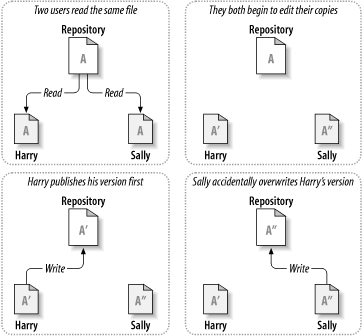
\includegraphics[width=.5\textwidth]{images/ch02dia2.png}
	~\cite{svnbook}
\end{center}

Yes, it's very much the same problem as when Harry was overwritten by Sally. And what did we do in this situation (as our first attempt)? We used the lock-modify-unlock model. And that's exactly what happens in a lot of software. Back to our earlier example:

\begin{verbatim}
lock(location);                         lock(location);
location.setX(5);                       location.setX(10);
location.setY(7);                       location.setY(0);
unlock(location);                       unlock(location);
\end{verbatim}


How the \texttt{lock} and \texttt{unlock} functions work is beyond the scope of this course (you will discuss them in operating systems). We just need to understand the concept of locking and unlocking data. When thread 1 locks the \texttt{location} object, it means thread 2's attempt to lock the same object cannot succeed until thread 1 unlocks the object. Thread 2 will therefore wait until the object is unlocked before proceeding. Similarly, if thread 2 gets to the lock first, thread 1 must wait for the lock to be released before it can make any changes. Either way, the result will be either $(5,7)$ or $(10,0)$, but it cannot be some mixup of the two like $(10, 7)$.

Relating all of this back to debugging: if you find some record or object that is in an inconsistent state (or some other kind of Heisenbug or shared data), then probably the error can be resolved with locking and unlocking the object.


\subsection*{Locking and Unlocking in Java}

\begin{quote}
\textit{``Knock knock.'' ``Race Condition.'' ``Who's there?''}
\end{quote}


In Java, there is a keyword that can be used to implement this lock-modify-unlock behaviour: \texttt{synchronized}. Let's examine proper use of this keyword, with information from the tutorial in~\cite{jenkov}. A synchronized block in Java is synchronized ``on'' some object. All synchronized blocks synchronized on the same object can only have one thread executing inside the synchronized area at the same time. All other threads attempting to enter the synchronized block must wait their turn.

We can apply the keyword to the following blocks:
\begin{enumerate}
	\item Instance methods
	\item Static methods
	\item Code blocks methods
\end{enumerate}

To make a method synchronized, just add the keyword \texttt{synchronized} to the function signature, such as: \texttt{public synchronized int foo()}. A synchronized instance method in Java is synchronized on the instance of the class. Thus if there are two instances, one thread can be in the synchronized block of each instance (so two threads). If the method is also static (e.g., \texttt{public static synchronized int bar()}) then they are synchronized on the class. If there are two instances of the class, only one thread can be inside method \texttt{bar} at a time. 

It's not necessary to make the entire method synchronized if we don't have to; in fact, the synchronized section should be as small as it can be. Suppose you have an object \texttt{s} that is shared between multiple threads. If you use the statement \texttt{synchronized(s)} the following block will be synchronized on that object \texttt{s}:
\begin{verbatim}
synchronized(s) {
    s.count++;
}
\end{verbatim}

At the line \texttt{synchronized(s)}, the this thread will try to get the lock. If someone has the lock, this thread will wait until the owner releases it and it is this thread's turn. If nobody else has the lock, or it becomes this thread's turn, it succeeds in getting the lock. Only once it has successfully acquired the lock can the code inside the braces execute. When execution reaches the closing brace of the synchronized block, the lock is released.

So let's take that technique and apply it to the location example from before:

\begin{verbatim}
synchronized(location) {                    synchronized(location) {
    location.setX(5);                           location.setX(10);
    location.setY(7);                           location.setY(0);
}                                          }
\end{verbatim}

The scenario that was a problem earlier occurred if a thread switch happened after the first thread set the X value and before it set the Y value. What happens in that scenario now that we have locks?

Thread one gets to the lock first. Nobody has the lock, so thread one gets it. Then, because it has the exclusive access to that lock, it can execute the code in the block, and it sets X to 5. At that time, we have a context switch and thread two runs. Because thread one has entered the synchronized block, thread two has to wait at the synchronized line for its turn. Then when thread one runs again, it sets Y to 7 and exits from the synchronized block (releasing the lock). Then, when thread two runs again, it can get the lock and it can update the location.


\section*{Debugging Embedded Systems: Challenges}
Embedded systems present a number of special challenges when it comes to debugging. Many of the challenges will result from the limitations of the system. For example, there may be no console output to print debugging messages, perhaps the debugger cannot be attached, or there might be no screen! There might also be difficulties with getting data into the system: how do you set up the environment you need?

\paragraph{First step.} Debug as much as you can separately, notably the
hardware and software. This may require:
\begin{itemize}
\item for software debugging: a hardware simulator;
\item for hardware debugging: test drivers and a test harness
\end{itemize}

Consider the following diagram:

\begin{center}
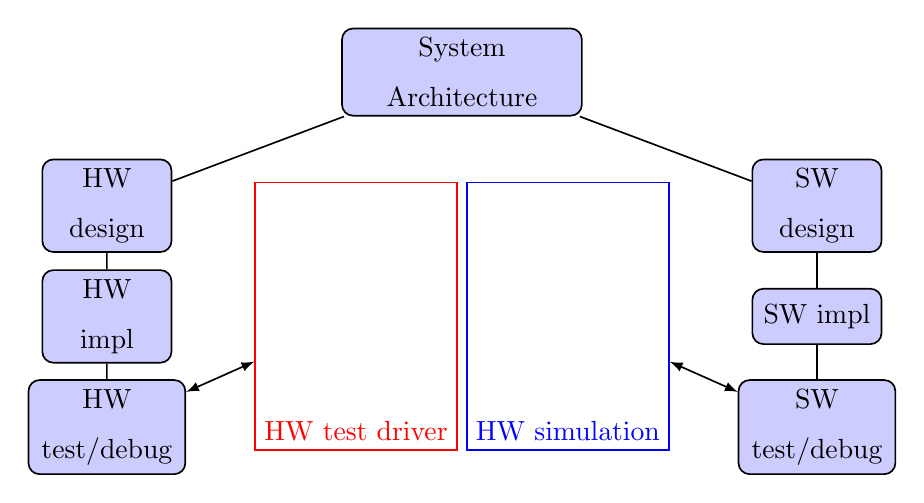
\begin{tikzpicture}[auto,node distance=4em,
                    semithick,initial text=]
  \node [bw,text width=8em] (arch) {System\\Architecture}; 

  \node [red,below left of=arch, xshift=-1em, draw, yshift=-6em, text height=9em] (hwtd) {HW test driver};
  \node [blue,below right of=arch, xshift=1em, draw, yshift=-6em, text height=9em] (swtd) {HW simulation};

  \node [bw, left of=hwtd,xshift=-5em,yshift=4em] (hwd) {HW design};
  \node [bw, below of=hwd] (hwi) {HW impl};
  \node [bw, below of=hwi,text width=5em] (hwt) {HW test/debug};

  \node [bw, right of=swtd,xshift=5em,yshift=4em] (swd) {SW design};
  \node [bw, below of=swd] (swi) {SW impl};
  \node [bw, below of=swi,text width=5em] (swt) {SW test/debug};

  \path[draw] (arch) -- (hwd)
        (arch) -- (swd)
        (hwd) -- (hwi)
        (swd) -- (swi)
        (hwi) -- (hwt)
        (swi) -- (swt);

   \path[draw,<->,>=latex] (hwt) -- (hwtd);
   \path[draw,<->,>=latex] (swt) -- (swtd);
\end{tikzpicture}
\end{center}

\paragraph{Debugging Challenges.} After you've integrated the hardware
and software, you'll face more challenges:

\begin{itemize}
\item \emph{fault (bug) localization}: Is the bug in the hardware or in the software? If it's in the software, which module is the problem? If it's in the hardware, which component is at fault?
\item \emph{need for instrumentation}: You'll need to add instrumentation to get diagnostic information. Print statements probably won't work, so you'll need 
to find some way of getting debug information from the software. And you'll
need to figure out how to determine the state of the hardware. At the
HW/SW interface, you can use a \emph{logic analyzer}.

Plan ahead and figure out how you'll instrument the system! (This separates the adults from the kids).

\item \emph{software breakpoints are hard}: If you use a breakpoint, then
it'll stop the software, but the embedded hardware continues to run (e.g.
think about the previous students' LEGO NXT robots: the software controlling the thing would stop, but the wheels would keep spinning...). Ideally, when a software breakpoint
occurs, ``freeze'' the hardware; this requires special support, which 
is hard to do.
\end{itemize}

\paragraph{Debugging of Field Problems.} Once you've deployed your
system, users will always find more problems. How do you diagnose
them?  This is a major challenge; you'll need to figure out how to get
initial diagnostic information. In aviation, the black box is one way
of getting diagnostic information from crashed aircraft. Windows
allows programs to upload diagnostic information upon crashes.


\subsection*{Strategies}
Let us now examine some strategies for debugging embedded systems.
 
\paragraph{Simulate.}
This is extremely helpful here: if we are able to reproduce the problem in a simulated environment (such as the Android emulator), then it will be much easier to debug. When working with the simulated environment we usually have console output and the ability to set breakpoints and walk through the code with the debugger. Unfortunately, however, sometimes problems do not appear in the simulation (or we don't have a simulation to work with, for whatever reason).
 
\paragraph{Use Your Actuators.}
As it is hard to get debug information out of an embedded system, you will have to make use of the actuators you have. You can make LEDs flash, or make the device beep (or another actuator available to you). If you only have a numeric display, perhaps show an error code that at least gives you a hint about what's gone wrong.

A famous example: the Power On Self Test (POST) from the BIOS. The POST would execute and then beep to indicate what, if anything, was wrong with the system. One beep meant all tests passed; different sequences of beeps indicated other issues: memory error, no boot device found, keyboard absent, etc. Once you identify what error code the system reported, you are closer to solving the problem.

\paragraph{Add Debugging Functions.}
Adding debugging functions to the system is one way to input specific debug data (or put the system in a state). These allow you to go around the normal rules of the system. Sometimes these are triggered with hardware. You might use a physical button (or sequence of button presses) to load some specific data into memory (or a function) to use in debugging. In other cases, you execute some software command(s) to trigger the debug function. Real life example: cheat codes (\texttt{iddqd}).

Normally, debugging functions are disabled when the system is released to the customers. But sometimes they are left in anyway (but behind security restrictions). 

\paragraph{Standard Interfaces.}
Joint Test Action Group (JTAG) is the common name for the IEEE 1149.1 Standard Test Access Port and Boundary-Scan Architecture. It is a standard interface for testing and I/O in many embedded systems. JTAG is used very frequently in commercial applications. It's possible (but not necessarily a good idea), to use the JTAG interface to flash your XBOX 360. In ECE~327, you'll learn more about how JTAG works. In this course, you don't need to know any details about JTAG. All you need to know is that it is an example of an embedded systems debugging standard.



\bibliographystyle{alpha}
\bibliography{155}


\end{document}

